% Appendix fragment: state-matched one-round response experiment.
% Requires: \usepackage{graphicx}
\subsection{State-matched response to advocacy}
\label{app:state-matched-response}

We isolate the one-round behavioral response of the population to controller advocacy while holding the epistemic population fixed. The experiment uses $N=24$ agents, $q=1$ social interaction, reasoning depth $L=2$, support redundancy $r=6$, recommendation-only control, and an incorrect controller target $Z$. We fix the sensing and actuation budgets to $q_c=b=18$ and explicitly initialize three target-support levels,
\[
 x_0\in\{0.25,0.375,0.50\},\qquad n_Z(0)\in\{6,9,12\}.
\]
Within each task, agent identities and initial knowledge sets $K_i(0)$ are identical across all three conditions, giving $\kappa_0=0.25$ and $\phi_0=0$. Target supporters are selected deterministically and balanced across the populated knowledge strata, with nested sets $Z_6\subset Z_9\subset Z_{12}$; all remaining agents are initialized at the correct relation. Thus only the initial social support for $Z$ changes across conditions.

For each $x_0$, we compare two deterministic one-round interventions: \textsc{Advocate}, in which the controller advocates for $Z$ at exactly $b=18$ controlled update positions, and \textsc{NoOp}, in which it does not intervene. The two arms use matched episode seeds. We evaluate two tasks with ten matched repetitions per task, yielding 120 one-round episodes. The sensor remains active for logging, but it does not determine the forced action.

The primary quantity is the signed intervention response
\begin{equation}
\chi(x_0)=\mathbb{E}[x_1-x_0\mid \mathrm{ADV},x_0]
-\mathbb{E}[x_1-x_0\mid \mathrm{NOOP},x_0],
\label{eq:state-matched-chi}
\end{equation}
with 95\% confidence intervals from 1000 bootstrap resamples of matched episode pairs. Since the action is deterministic within each arm, this experiment estimates a response contrast rather than an action-to-population mutual information.

\begin{figure}[t]
    \centering
    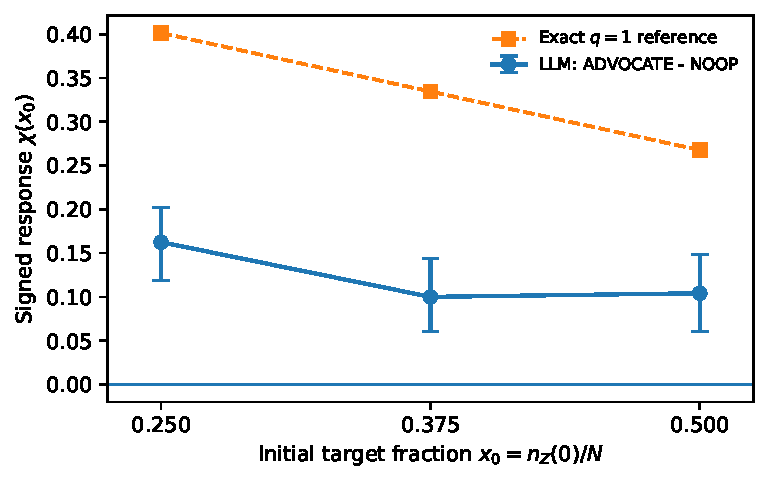
\includegraphics[width=\columnwidth]{figures/state_matched_response.pdf}
    \caption{One-round state-matched response to advocacy. Points show the empirical \textsc{Advocate}-minus-\textsc{NoOp} response with 95\% matched-pair bootstrap intervals. The dashed curve is the exact $q=1$ reference at $N=24$ and $b=18$, $\chi_{q=1}(x_0)=(1-x_0)[1-(1-1/N)^b]$. Advocacy produces a positive response at every imposed initial target fraction, while the response does not increase with pre-existing target support over the tested range.}
    \label{fig:state-matched-response}
\end{figure}

The measured responses are $\chi(0.25)=0.163$ (95\% CI $[0.119,0.202]$), $\chi(0.375)=0.100$ ($[0.060,0.144]$), and $\chi(0.50)=0.104$ ($[0.060,0.148]$). The controller therefore produces a positive causal shift toward its target at all three matched states. However, the largest response occurs at the lowest tested target fraction, and increasing the initial target support from $x_0=0.375$ to $0.50$ produces no additional gain. The exact $q=1$ reference predicts the same qualitative ordering---largest leverage at low target support---but substantially larger responses ($0.401$, $0.334$, and $0.268$, respectively). Thus, in this controlled one-round setting, LLM advocacy is effective but markedly weaker than the idealized copying reference, and there is no evidence that additional pre-existing social support amplifies the intervention response.
